%['国际 石油', '价格', '攀高_1', '', ''] --> ['橡胶', '价格', '上升_1', '', '']
%['X0', '价格', '攀高_1', '', ''] --> ['X1', '价格', '升高_1', '', ''] [1]
%X0 ['化石燃料', '污染物', '原料', '耗才', '行业']
%X1 ['弹性材料', '天然聚合物', '产品', '材料', '行业', '柔性材料']
%1 :
%X0 madeof X1
%
%11
%['', '乙醇', '增长_1', '', ''] --> ['玉米', '价格', '上涨_1', '', '']
%['', 'X0', '增加_1', '', ''] --> ['X1', '价格', '升高_1', '', ''] [1]
%X0 ['醇', '生物燃料', '烷醇', '极性溶剂']
%X1 ['谷类', '粮食', '植物油', '厂']
%1 :
%X0 relatedto X1
%



\section{Approach}
\label{sec:approach}

\subsection{Overview}
\begin{figure*}[htbp]
	\centerline{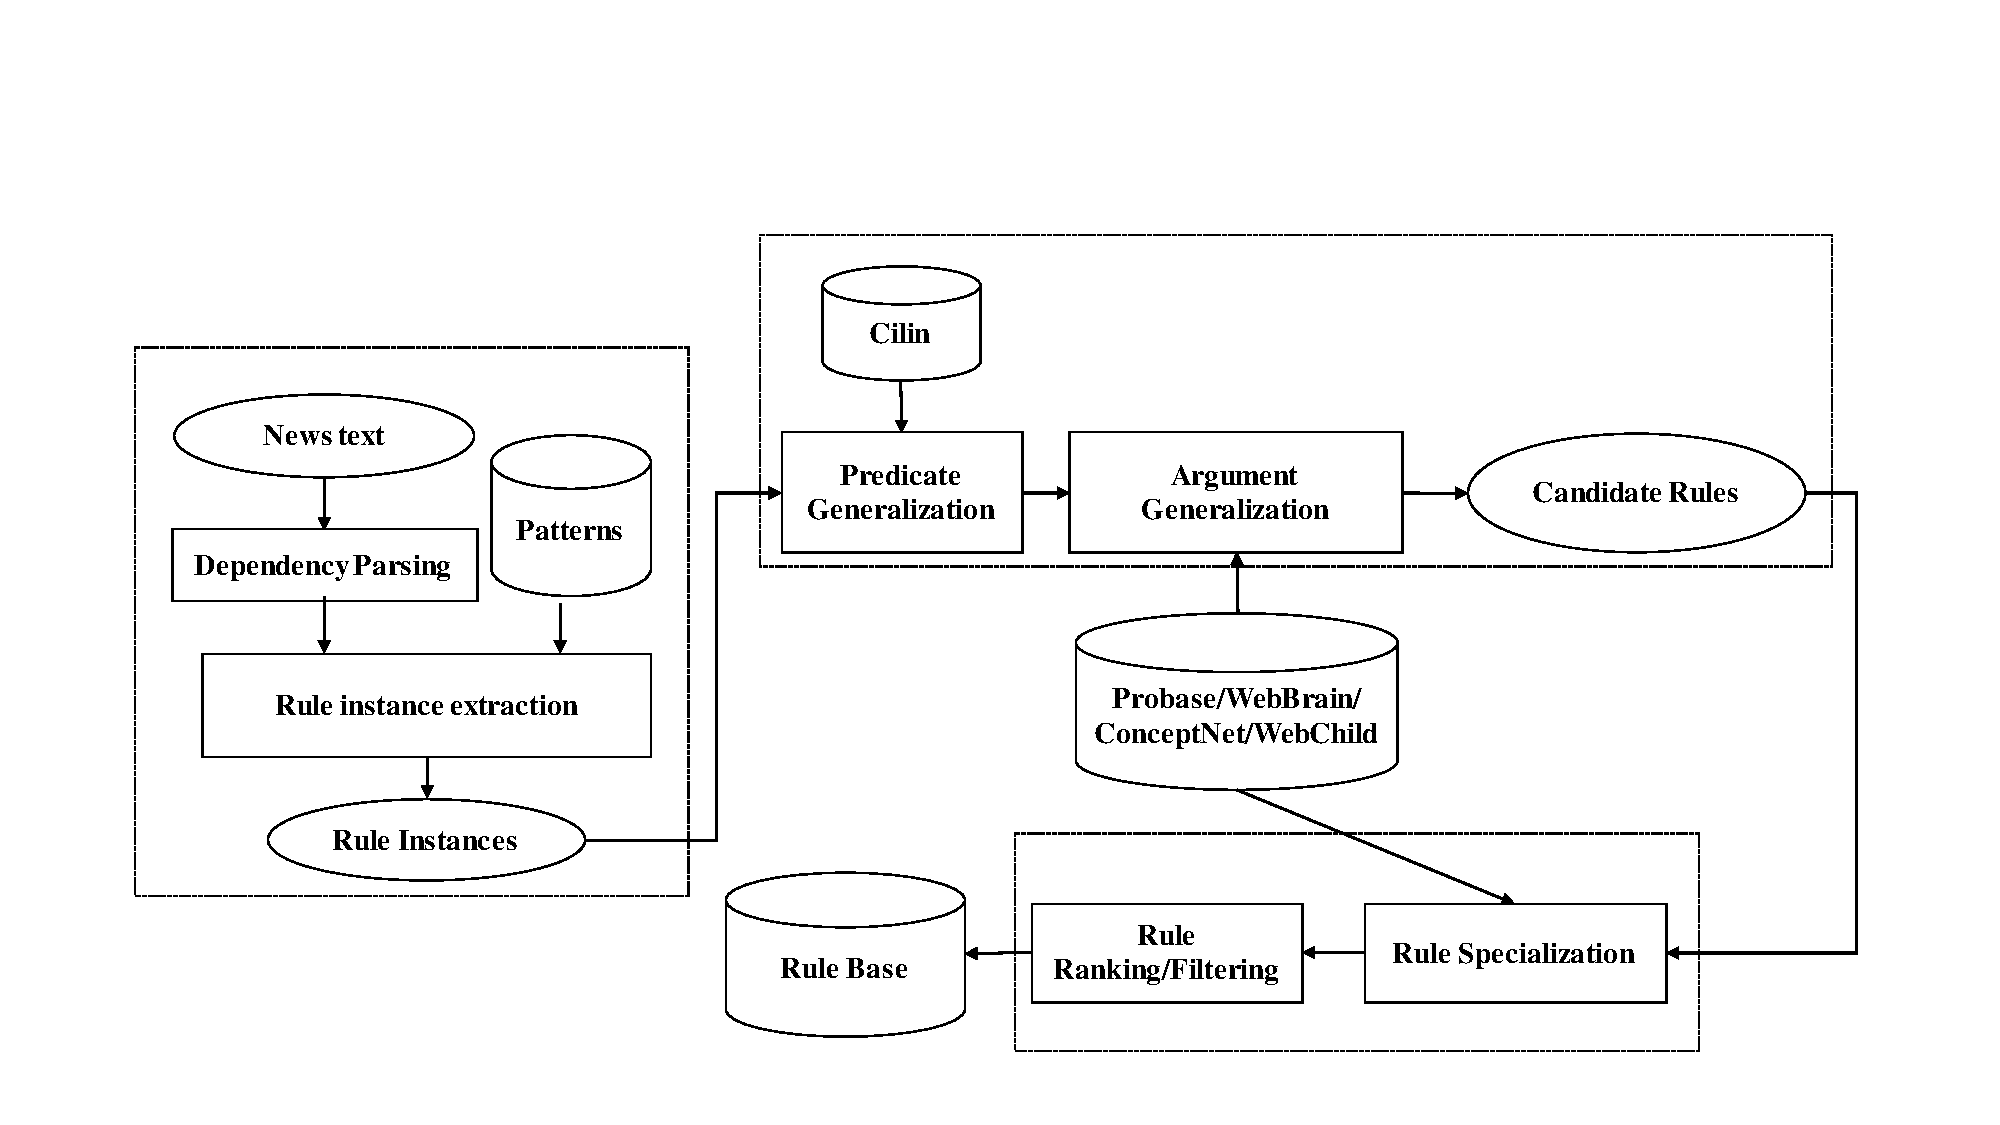
\includegraphics[width=\textwidth]{figures/approach}}
	\caption{Overview of our proposed framework.}
	\label{fig:approach}
\end{figure*}
%introduction 多介绍why
%approach 多介绍how

Figure \ref{fig:approach} describes our proposed novel framework. Generally, it consists of four key submodules: rule instances extraction, constructing a knowledge base, rule generalization and rule specialization. Rule instances extraction submodule mainly extracts the structured causality event pairs (also called rule instances) from large liberal text. Constructing a knowledge base submodule is a auxiliary module for rule generalization submodule and rule specialization module, mainly due to the lack of Chinese resources. Rule generalization submodule generalizes the extracted rule instances to candidate rules resorting to the newly built knowledge base. Rule specialization submodule mainly focuses on adding relation constraints between arguments in the the candidate rules by alleviating their generalization ability to make rules reasonable. \TD{and also includes rule filtering, and rule ranking.}

\subsection{Rule Instances Extraction }
Causality is expressed by natural language texts and can be identified by linguistic patterns known as the causal cues \cite{chang2004causal}.

\begin{table}[htbp]
	\caption{Causal patterns. A is a cause tokens span, and B is an effect tokens span. Word '因为' represents a group works like '由于,'是因为','因为','缘于','归因于','原因是','起因','鉴于', word '且' represents a group of words like '并且','而且','同时','且','与此同时' and word '所以' represents a group of words like '所以','因而','因此','故此','故而','因故','导致','招致','以致','引致','诱致','致使','造成','使得','从而','从而使','于是','为此'}
	\begin{center}
		\begin{tabular}{|c|c|} \hline
			\textbf{Pattern}& \textbf{Priority}\\ \hline
			因为 $A_1$, 且 $A_2$,所以 $B_1$  且 $B_2$& 0\\ \hline
			因为 A,所以 $B_1$ 且 $B_2$&1\\ \hline
			因为 $A_1$, 且 $A_2$, 所以 B&2\\ \hline
			因为 A, 所以B&3\\ \hline
			A,所以 B&4\\ \hline
			因为 A,B&5\\ \hline
		\end{tabular}
		\label{tab:causal_pattern}
	\end{center}
\end{table}	

Firstly, we construct a set of causal patterns to extract cause span and effect span. The casual patterns are shown in Table \ref{tab:causal_pattern}. All the causal patterns can be divided into 5 groups based on the pattern structure. Each group of causal patterns follow the template of \textit{Expression, Priority}. Each pattern consists of a regular expression and priority which is regarded as the matching order when several causal patterns are matching one sentence. We arrange the priority based on the causality precision. The more precise the extracted causality information is, the higher-priority it should be, correspondingly, the smaller the number it would be. For instance, '因为... 所以...' captures more precise information than '因为 A, B' when matched, so it is prior. 
%
%Alternatively, we can use a more sophisticated way to catch the causality such as \cite{zhao2016event}. In this study, however, we focus more on the precision of causality extraction rather than the recall using more complex patterns, also we think a more sophisticated method used on such noisy text may lead to more errors.
%
Exploiting these causal patterns, we can extract pairs of causal spans. Then, we take advantage of existing parser tool\cite{manning2014stanford} to extract the cause event and effect event to make up the rule instances. In fact, we use the parser to parse the sentences first, then use these causal patterns to extract the rule instances. Since most sentences have no casual cues and parsing is a very time-consuming operation, we firstly filter out the sentences without casual patterns as a preprocessing.

This submodule will be illustrated using the following examples. Consider the following sentences:
\begin{enumerate}[\IEEEsetlabelwidth{12)}]
	\item 但由于国际石油价格一路攀高一直到现在创纪录的每桶五十几美元,导致目前合成橡胶价格快速上升,已经超过天然橡胶,像丁苯橡胶已从年初的每吨11000元上涨到现在的14000元。\\
	
	\item 2005年我国乙醇汽油消费玉米1300万吨,预计2006年消费玉米1600万吨,由于石油涨价,乙醇转化用粮需求将会快速增长,从而拉动玉米价格上涨。	
\end{enumerate}

\textbf{Firstly.} Feed each sentence into parser tool, then join the  segmented	 output tokens with blanks. For sentence (1), We will get "但 由于 国际 石油 价格 一路 攀高 一直 到 现在 创 纪录 的 每 桶 五十几 美元 , 导致 目前 合成 橡胶 价格 快速 上升 , 已经 超过 天然 橡胶 , 像 丁苯 橡胶 已 从 年初 的 每 吨 11000 元 上涨 到 现在 的 14000 元 。". Then we exploit the elaborate patterns to match the padded sentence and we can get cause tokens span "国际 石油 价格 一路 攀高 一直 到 现在 创 纪录 的 每 桶 五十几 美元" and the effect tokens span "目前 合成 橡胶 价格 快速 上升 , 已经 超过 天然 橡胶 , 像 丁苯 橡胶 已 从 年初 的 每 吨 11000 元 上涨 到 现在 的 14000 元 。".

\textbf{Secondly.} After deriving the cause tokens span and effect tokens span, we further extract the cause event and effect event to make up the rule instance. The events in rule instances are mediated by predicate, namely verb, so we regard every verb token in the tokens span as a predicate. Then, we find the corresponding subject and object of each predicate. Here, we can get subject and object of each predicate beyond the scope of its belonging event's tokens span which is an advantage of parsing the whole sentence before matching the cause effect spans since it can alleviate the parsing error by feeding more context information into the parser. Last, we get the Compound nouns of subject and object with the dependency relation of 'compound:nn', which can be also beyond the scope of its belonging token spans. These compound nouns are placed at the event as the same order appeared in their origin sentence. Since it may be more than one predicates in cause tokens span or effect tokens span, which means we can get more than one structured events from cause tokens span or effect tokens span, we do a combination of the cause events and effect events to get more rule instances. We believe that the right rule instances will be appeared more often than the corrupted. Also, later, we will rank the low frequency pairs into the back and filter the undesired rule. From sentence (1), we can get many rule instances, one desired rule instance is ('国际 石油', '价格', '攀高\_1', '', '')$->$('橡胶', '价格', '上升\_1', '', ''). From sentence (2), we can get many rule instances, ('', '乙醇', '增长\_1', '', '')$->$('玉米', '价格', '上涨\_1', '', '') is our desired. Meanwhile we also consider the neg relation of the predicate, we mark it behind predicate, which is a small implement trick. '\_0' means the predicate is negative, while '\_1' means the predicate is positive.


\subsection{Constructing Knowledge Base}
From above rule instance extraction submodule, We can get a rule instances repository. With such huge specific rule instances, we hope to further discover the powerful knowledge hidden in these rule instances. 
so we generalize such a large amount rule instances with a more general form. As discussed in Section \ref{sec:intro}, we need to build such a knowledge base. Taxonomy and common sense are two major kinds of knowledge in such knowledge base.

\textbf{Taxonomy.} Taxonomy is composed of IsA relation instances. We have investigated the CN-Probase\cite{b1}, But It even can't find the concept of common entities like '橡胶','中国'. As discussed in Section \ref{sec:intro}, we decide to enlarge the chinese taxonomy. Firstly, we collect the items from Probase, the items with 'IsA' relation in ConceptNet5, and the items with IsA relation in Webbrain. Then, we fuse them together, since Probase is a probabilistic taxonomy, we also assign a constant probability to the items from WebBrain, ConceptNet. Lastly, we translate them into Chinese with google translator. \TD{[做一个脚注 说一下方法 context]}   

\textbf{Common sense.} Commonsense relations between arguments are used in rule specialization submodule to make rules reasonable. There exist many commonsense knowledge bases such as ConceptNet5, WebBrain, WebChild.  The numbers of the relations in these knowledge bases are limited. And some relations are equivalent among different knowledge bases, such as '/r/RelateTo' in ConceptNet is equivalent to 'relateto' in WebBrain. So we normalize all the relations names literally.

% Meanwhile, many pairs of arguments have more than one relations which are  duplicated semantically. For example, (sweet corn, corn) has the relations 'relatedto' and 'partof', obviously, 'partof' consists of 'relatedto' semantically. So we hope to remove the semantic reduplication relations. which means we need find the semantic containment relations among these relations.

%Algorithm \ref{alg:alg1} shows the Relations Containment algorithm we proposed. It firstly counts each relation and its corresponding arguments pairs. Then, compare the every two correlated relations, and record their containment relation. Last, enumerate all relations in each pair of arguments, remove the relation which is not contained in other relations existed in this pair of arguments.
 
%\begin{algorithm}
%	\caption{Relations Containment  \label{alg:alg1}} 
%	\KwIn{ commonsense triples $TS = \{t_1, t_2, ..., t_n\}$, ~$t_i = (arg_i1, rel, arg_i2)$ } 
%	\KwOut{ Relations Containment Relations $RCR$}
%	RCR $\leftarrow$ []\\
%	ERs $\leftarrow$ defaultdict(set)\\
%	REs $\leftarrow$ defaultdict(set)\\
%	\For{$t_i \ in \ TS$}{
%	$arg_i1,rel,arg_i2 \leftarrow  t_i$\\
%		REs[$rel$].add(($arg_i1,arg_i2$))	\\
%		ERs[($arg_i1,arg_i2$)].add(rel)	
%	}
%	\For {$rels \ in \ ERs.values()$}{
%		\For{$rel_1, rel_2 \in rels$}{
%	$P( rel_1|rel_2 )=\frac{|REs[rel_1 ] \cap  REs[ rel_2 ]|}{|REs[ rel_2 ]|}$\\
%	$P( rel_2|rel_1 )=\frac{|REs[ rel_1 ] \cap  REs[ rel_2 ]|}{|REs[ rel_1 ]|}$\\
%			\If{$P(rel_1|rel_2) > P(rel_2|rel_1)$}{
%				RCR.append(($rel_1, rel_2$))\\
%				remove $rel_1$	from $rels$
%			}\Else{
%				RCR.append(($rel_2, rel_1$))\\
%				remove $rel_1$	from $rels$
%			}
%		}
%	}
%	\Return RCR, ERs
%\end{algorithm}

When fusing these knowledge bases, we regard arguments from different knowledge bases which have the same literal name as the same arguments.
s
\subsection{Rule Generalization}
with the knowledge base, now, we can generalize the rule instances extracted from rule instances extraction submodule into candidate rules to represent more general knowledge. For example, we hopefully generalize from each cluster of rule instances to one candidate rule. For example, given two rule instances in one cluster, ('国际 石油', '价格', '攀高@攀高', '', '') $->$ ('橡胶', '价格', '上升@升高', '', '') and ('国际 柴油', '价格', '攀高@攀高', '', '') $->$ ('橡胶', '价格', '上升@升高', '', ''), the generalized candidate rule would be('X0', '价格', '攀高', '', '') $->$ ('X1', '价格', '升高', '', '') where 'X0' IsA' 化石燃料','原料' and  'X1' IsA '弹性材料' '天然聚合物'.

We divide the rule generalization into two steps:
\subsubsection{Predicate Generalization}
Different literal predicates may express the same meaning. predicates like 'raise','rise,','soar,','increase,','gain,','enhance' would express the same meaning, so we use the Ciling to canonicalize the predicates. Ciling is the largest word-level Chinese synonym resource, which split the Chinese words into groups according to the relevance of these words. For each group, we choose most frequently appeared one in our text to represent this group of words.

\subsubsection{Argument Generalization}
After predicate generalization, we wish to generalize each cluster of similar rule instances to one candidate rule, since one candidate rule should be supported by more than one rule instance. Algorithm \ref{alg:alg2} describes the procedure, mainly consists of two components, clustering and conceptualization.
The input of this overall algorithm is rule instances, and our built knowledge base, our desired output is candidate rules.

\textbf{Clustering.} This procedure is shown in Algorithm \ref{alg:alg2}. We firstly iterate each rule instance, and find its similar rule instances , then gather them to make up a cluster. Variable RICs reserves all the rule instances clusters. As for the $Similar$ function, which is used to decide whether two rule instances should be gather together into one cluster. The basic idea is that if the arguments can't be conceptualized, They must be the same literally, else we use the word embedding to calculate their similarity. Only when the similarity value is larger than a specified threshold, we gather them together.

%Given two rule instances, If both arguments in the same argument type(subj,obj, compound nouns,predicate) can't be conceptualized, if they are the same, these two rule instacnes are similar, else they are not similar. If both arguments can be conceptualized, We will exploit the word embedding to measure their similarity. specifically, we concatenate all the conceptualized arguments, last we calculate the cosine similarity. If it is great than a threshold, we regard these two rule instances similar, otherwise they are not similar.   

\textbf{Argument Conceptualization.} After get clusters of rule instances, we need generalize each cluster of rule instances into one candidate rule. Algorithm \ref{alg:alg2} line 10 to line 24 shows this process. the generalization can be divided into several argument conceptualization part. Figure \ref{fig:argument_generalization} shows one of them. in the left part is a cluster of given arguments and their respective conceptualization, and in the right part is common concepts satisfy all the arguments and also we remove the very general concepts. After doing several argument conceptualizations in this rule instances cluster, we can get a candidate rule.

We use all the news text we crawled to train the word embedding with word2vec tool \footnote{ \url{ https://code.google.com/archive/p/word2vec}}, the output vector dimension is 400. 
%which includes single rule instance argument generalization in the left part, and arguments generalization in rule instances cluster in the right part. the blue part is the least general generalization in concept space of the argument. 


%\textbf{argument generalization of single rule instance.} rule instance argument generalization use external knowledge to generalize the entities in the rule instance, Here We also make a lexicon, which can prevent some abstract entities from conceptualization, For example, ('橡胶', '价格', '上升@升高', '', '') we want generalize '橡胶' rather than price, So we make a concrete lexicon which consist all the leaf nodes of the IsA relations in ConceptNet5, Since we observe the entities in ConeptNet5 are more concrete.

%\textbf{argument generalization of rule instances cluster.}one candidate rule is always derived after observing a cluster of similar rule instances. So we hope to gather clusters of generalized rule instances to generalize candidate rules. Algorithm 2 describe how to generalize each candidate rule from each cluster of generalized rule instances. Generally, we first generalize every rule instances, Then for each generalized rule instance, we find the similar rules which can be clustered together, then we generalize cluster of rule instances to one candidate rule, Repeat until process all generalized rule instances, Last we can get the candidate rules. 

\begin{figure}[htbp]
	\centerline{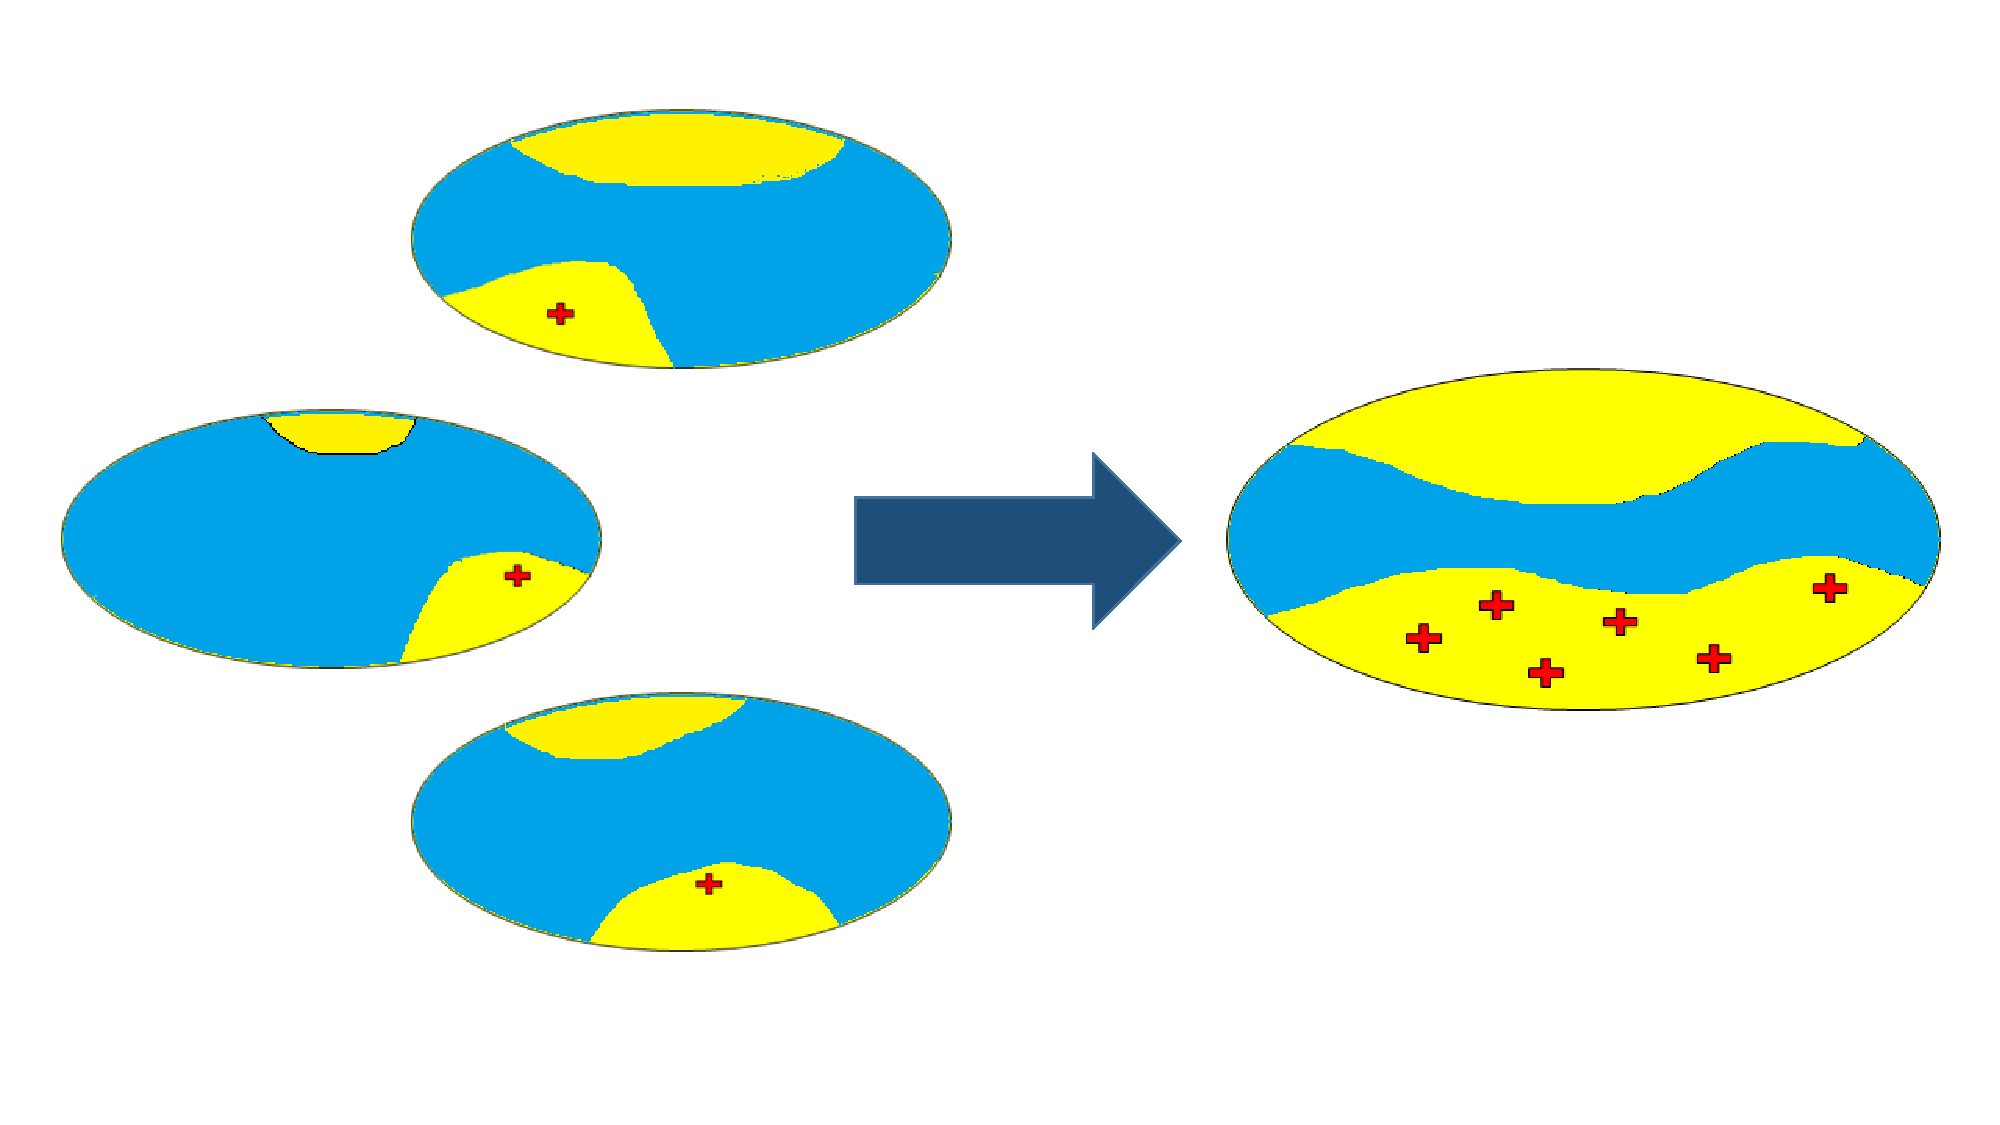
\includegraphics[width=0.9\columnwidth]{figures/argument_generalization}}
	\caption{Argument Generalization.}
	\label{fig:argument_generalization}
\end{figure}


\begin{algorithm}
	\caption{Rule Argument Generalization.\label{alg:alg2}} 
	\KwIn{ Generalized Rule Instances} 
	\KwOut{Candidate Rules}
	initiate $RIS \leftarrow $all generalized rule instances\\
	$RICs \leftarrow []$\\
	$CRs \leftarrow []$\\
	\For{$ri_i \in RIs$}{
		initiate $ric \leftarrow [ri_i]$, Remove $ri_i$ from RIs\\
		\For{$ri_j \in RIs$}{
			\If{Similar$(ri_i,ri_J)$}{
			$ric.append(ri_j)$ \\
			Remove $ri_j$ from $RIs$
			}
		$RICs.append(ric)$
		}
	}
	\For {each cluster $ric \in RICs$}{
		rule $\leftarrow$ null\\
		\For{echo position i in the rule}{
			\eIf{Argument in position i is conceptualized}{
				$e_{i1},e_{i2},...,e_{ik}$ are the conceptualized entities in position i from cluster $ric$\\
				 their conpcets are $Cs_{i1},Cs_{i2},...,Cs_{ik}$ \\
				$Cs_i=Cs_{i1}\cap Cs_{i3} ... \cap Cs_{ik}$\\
				\For{$c_i,c_j \in Cs_i$}{
					\If{Overlap($c_i,c_j$)}{
					Remove $c_m$ from $Cs_i$, where $c_m= argmax_m{|E_{ci}|,|E_{cj}|}$
					}
				}
			rule[position i]=$Cs_i$
			}
		 {
			rule[position ]=argument in position i
		}
	  CRs.apppend(rule)
	}
	\Return CRs 
	}
	\SetKwFunction{FM}{Similar}
	\SetKwProg{Fn}{Function}{:}{}
	\Fn{\FM{$ri_1$, $ri_2$}}{
		initiate Vector1=array(), Vector2=array()\\
		\For{$argument_type$ in $NSPNO$}{
			$arg_1=ri_1[argument_type]$
			$arg_2=ri_2[argument_type]$\\
			\eIf{$arg_1$ can be conceptualized \& $arg_2$ can be conceptualized}
			{
				Vector1.concatenate($WordEmbedding_{arg_1}$)
				Vector2.concatenate($WordEmbedding_{arg_2}$)
			}{
				\KwRet $False$
			}
		}
		$sim=Cosine(Vector1,Vector2)$\\
		\eIf{$sim>0.4$}{
			\KwRet $True$
		}{
			\KwRet $False$
		} 
	} 
	\SetKwFunction{FC}{Overlap}
	\SetKwProg{Fn}{Function}{:}{}
	\Fn{\FC{$c_1$, $c_2$}}{
		initiate $I_c_1 \gets$ the instances of $c_1$ in knowledge base
		initiate $I_c_2 \gets$ the instances of $c_2$ in knowledge base
		\eIf{$\frac{|I_c_1 \cap I_c_2|}{min(|I_c_1|,|I_c_2|)}>0.2$}{
			\KwRet $True$
		}{
			\KwRet $False$
		} 
	} 
\end{algorithm}	

\subsection{Rules Specialization.}
Rule generalization step tries to make candidate rules more general than rule instances, but such rule generalization makes the candidate rules look unreasonable even wrong as discussed in Section \ref{sec:intro}. So we further add relation constraints to specialize the candidate rules aiming at getting reasonable rules.

Here, we exploit our built knowledge base to find all the relations between each pair arguments separately in cause event and effect event.
Take an example, there are many arguments $a_1, a_2$ in subject position of cause event, and $a_3, a_4$ in object position of effect event. We will firstly find all the relations between one argument in $a_1,a_2$ and the other argument in $a_3,a_4$. Then, we will fetch the most commonly appeared relations as one of the relation constraints between subject in cause event and object in effect event.
After adding get these relations constraint into the candidate rules, we will get the final rules.

% Sometimes these relations may not be the same literally, but they are semantically duplicated, which will also regarded as the same relation to increase the count. After adding get these relations constraint into the candidate rules, we will get the final rules.


%For example, Conceptualizing one argument to a concept make the rule much more general, ('国际 石油', '价格', '攀高@攀高', '', '') $-->$ ('橡胶', '价格', '上升@升高', '', '') to('X0', '价格', '攀高', '', '') $-->$ ('X1', '价格', '升高', '', '') where 'X0' IsA'化石燃料''X1' IsA '产品', For instance, coal IsA '化石燃料',phone IsA '产品', We instance X0 and X1 respectively with coal and phone. Then the rule means  raising the price of coal would lead to the rubber's rising, Which is obviously unreasonable. 

%So we hopefully find the relation constraint between X0 and X1, also we want to discover the relation between X0, X1 is X0 'madeof' X1. and mostly the relations are commonsense relation. 
%
%Here, we find all the relations between each pair arguments in cause event and effect event from our built knowledge base, which may consist many pair of arguments, and many relations of one pair arguments. since one rule contains many rule instances, Here, We would like the intersect these relations which include the relation's semantic duplication, the remaining relations will be kept as the relation constraint in this rule. 

%\begin{equation}
%\label{relation_saliency}
%RS_{ij}=\frac{Count(rel_i,R_j)}{Count(R_j)}
%\end{equation}
%pick $rel_i$ for $R_j$ as relation constraint, where $i=argmax_i RS_{ij}$

%\subsubsection{  Filter and Ranking.}
